\documentclass[12pt,addpoints]{repaso}
\grado{4}
\nivel{Primaria}
\cicloescolar{2024-2025}
\materia{Matemáticas}
\unidad{1, 2 y 3}
\title{Practica la Unidad}
\aprendizajes{\tiny
      \item Expresa oralmente la sucesión numérica hasta cuatro cifras, en español y hasta donde sea posible, en su lengua materna, de manera ascendente y descendente a partir de un número natural dado.
      \item Representa, con apoyo de material concreto y modelos gráficos, fracciones: medios, cuartos, octavos, dieciseisavos, para expresar el resultado de mediciones y repartos en situaciones vinculadas a su contexto.
      \item Resuelve situaciones problemáticas vinculadas a su contexto que implican sumas o restas de números naturales de hasta cuatro cifras utilizando los algoritmos convencionales y números decimales hasta centésimos, con apoyo de material concreto y representaciones gráficas.
	  \item Resuelve situaciones problemáticas que implican sumas o restas de fracciones con diferente denominador (tercios, quintos, sextos, novenos y décimos) vinculados a su contexto, mediante diversos procedimientos, en particular, la equivalencia.
	  \item Resuelve situaciones problemáticas vinculadas a su contexto que implican multiplicaciones de números naturales de hasta tres por dos cifras, a partir de diversas descomposiciones aditivas y el algoritmo convencional y el uso de un algoritmo para dividir números naturales de hasta tres cifras entre un número de una o dos cifras; reconoce al cociente y al residuo como resultado de una división.
	  }
\author{Melchor Pinto, JC}
\begin{document}
\INFO
\begin{questions}
	\questionboxed[2]{Escribe sore la línea los siguientes números

		\begin{multicols}{2}
			\begin{parts}\large
				\part  \fillin[$14005$][1.1cm] Catorce mil cinco.
				\part  \fillin[$11524$][1.1cm] Once mil quinientos veinticuatro.
				\part  \fillin[$13642$][1.1cm] Trece mil seiscientos cuarenta y dos.
				\part  \fillin[$10189$][1.1cm] Diez mil ciento ochenta y nueve.
				\part  \fillin[$13990$][1.1cm] Trece mil novecientos noventa.
				\part  \fillin[$11300$][1.1cm] Once mil trescientos.
				\part  \fillin[$14400$][1.1cm] Catorce mil cuatrocientos.
				\part  \fillin[$12881$][1.1cm] Doce mil ochocientos ochenta y uno.
				\part  \fillin[$10711$][1.1cm] Diez mil setecientos once.
				\part  \fillin[$11740$][1.1cm] Once mil setecientos cuarenta.
				\part  \fillin[$10298$][1.1cm] Diez mil doscientos noventa y ocho.
				\part  \fillin[$13422$][1.1cm] Trece mil cuatrocientos veintidos.
			\end{parts}
		\end{multicols}
	}
	% \section*{\ifprintanswers{Números romanos                                }\else{}\fi}
	% \subsection*{\ifprintanswers{Números romanos 1                              }\else{}\fi}
	% \subsection*{\ifprintanswers{Números romanos 2                              }\else{}\fi}
	% \subsection*{\ifprintanswers{Números romanos 3                              }\else{}\fi}
	% \subsection*{\ifprintanswers{Números romanos 4                              }\else{}\fi}
	% \subsection*{\ifprintanswers{Números romanos 5                              }\else{}\fi}
	\questionboxed[2]{Escribe el valor de los siguientes números romanos

		\begin{multicols}{4}
			\begin{parts}\large
				\part \fillin[$16$][1cm] XVI
				\part \fillin[$482$][1cm] CDLXXXII
				\part \fillin[$18$][1cm] XVIII
				\part \fillin[$98$][1cm] XCVIII
				\part \fillin[$64$][1cm] LXIV
				\part \fillin[$199$][1cm] CXCIX
				\part \fillin[$36$][1cm] XXXVI
				\part \fillin[$42$][1cm] XLII
				\part \fillin[$37$][1cm] XXXVII
				\part \fillin[$63$][1cm] LXIII
				\part \fillin[$29$][1cm] XXIX
				\part \fillin[$34$][1cm] XXXIV
			\end{parts}
		\end{multicols}
	}

	\questionboxed[2]{Escribe en números romanos los siguientes números

		\begin{multicols}{4}
			\begin{parts}\large
				\part 38  \fillin[XXXVIII][2.5cm]
				\part 150 \fillin[CL][2.5cm]
				\part 82  \fillin[LXXXII][2.5cm]
				\part 199 \fillin[CXCIX][2.5cm]
				\part 46  \fillin[XLVI][2.5cm]
				\part 98  \fillin[XCVIII][2.5cm]
				\part 482 \fillin[CDLXXXII][2.5cm]
				\part 28  \fillin[XXVIII][2.5cm]
				\part 45  \fillin[XLV][2.5cm]
				\part 94  \fillin[XCIV][2.5cm]
				\part 308 \fillin[CCCVIII][2.5cm]
				\part 40  \fillin[XL][2.5cm]
			\end{parts}
		\end{multicols}
	}

	% \section*{\ifprintanswers{Sistema decimal                                }\else{}\fi}
	% \subsection*{\ifprintanswers{Posicionamiento decimal 1                      }\else{}\fi}
	% \subsection*{\ifprintanswers{Posicionamiento decimal 2                      }\else{}\fi}

	\questionboxed[2]{Señala la opción que responda correctamente a cada una de las siguientes preguntas:

		\begin{multicols}{2}
			\begin{parts}\large
				\part ¿Qué lugar ocupa el 6 en 6418?     \fillin[C][0.5cm]
				\part ¿Qué lugar ocupa el 2 en 206418?   \fillin[A][0.5cm]
				\part ¿Qué lugar ocupa el 2 en 87264?    \fillin[D][0.5cm]
				\part ¿Qué lugar ocupa el 1 en 1681?     \fillin[F][0.5cm]
				\part ¿Qué lugar ocupa el 1 en 6138?     \fillin[D][0.5cm]
				\part ¿Qué lugar ocupa el 8 en 198114?   \fillin[C][0.5cm]
				\part ¿Qué lugar ocupa el 7 en 46878?    \fillin[E][0.5cm]
				\part ¿Qué lugar ocupa el 4 en 149778?   \fillin[B][0.5cm]
			\end{parts}

			\columnbreak%

			\begin{choices}\Large
				\choice {\color{red}centenas de millar.}
				\choice {\color{blue}decenas de millar.}
				\choice {\color{Goldenrod}unidades de millar.}
				\choice {\color{red}centenas.}
				\choice {\color{blue}decenas.}
				\choice {\color{Goldenrod}unidades.}
			\end{choices}
		\end{multicols}
	}

	% \subsection*{\ifprintanswers{Notación desarrollada 1                        }\else{}\fi}
	% \subsection*{\ifprintanswers{Notación desarrollada 2                        }\else{}\fi}


	\questionboxed[4]{Escribe la notación desarrollada de cada uno de los siguientes números:

		\begin{multicols}{2}
			\begin{parts}\Large
				\part $15984=$ \fillin[$10000+5000+900+80+4$][2.4in]
				\part $4936 =$ \fillin[$4000+900+30+6$][2.4in]
				\part $27545=$ \fillin[$20000+7000+500+40+5$][2.4in]
				\part $6215 =$ \fillin[$6000+200+10+5$][2.4in]
				\part $5454 =$ \fillin[$5000+400+50+4$][2.4in]
				\part $6451 =$ \fillin[$6000+400+50+1$][2.4in]
				\part $19679=$ \fillin[$10000+9000+600+70+9$][2.4in]
				\part $26324=$ \fillin[$20000+6000+300+20+4$][2.4in]
				\part $5717 =$ \fillin[$5000+700+10+7$][2.4in]
				\part $31126=$ \fillin[$30000+1000+100+20+6$][2.4in]
				\part $4818 =$ \fillin[$4000+800+10+8$][2.4in]
				\part $7145 =$ \fillin[$7000+100+40+5$][2.4in]
			\end{parts}
		\end{multicols}
	}

	% \subsection*{\ifprintanswers{Posicionamiento decimal y Notación desarrollada}\else{}\fi}

	\questionboxed[2]{Señala la opción que responda correctamente a cada una de las siguientes preguntas:

		\begin{multicols}{2}
			\begin{parts}\large
				\part En el número 3658, ¿qué número ocupa la posición de las decenas?

				\begin{oneparcheckboxes}
					\choice 3 \CorrectChoice 5 \choice 6 \choice 8 \choice 9
				\end{oneparcheckboxes}

				\part En el número 17542, ¿qué número ocupa la posición de las unidades de millar?

				\begin{oneparcheckboxes}
					\choice 1 \CorrectChoice 7 \choice 5 \choice 4 \choice 2
				\end{oneparcheckboxes}

				\part En el número 5984, ¿qué número ocupa la posición de las centenas?

				\begin{oneparcheckboxes}
					\choice 4 \choice 2 \choice 5 \choice 8 \CorrectChoice 9
				\end{oneparcheckboxes}

				\part En el número 7841, ¿qué número ocupa la posición de las decenas?

				\begin{oneparcheckboxes}
					\choice 1 \choice 7 \choice 8 \CorrectChoice 4 \choice 2
				\end{oneparcheckboxes}

				\part En el número 3918, ¿qué número ocupa la posición de las centenas?

				\begin{oneparcheckboxes}
					\choice 3 \choice 1 \choice 6 \choice 8 \CorrectChoice 9
				\end{oneparcheckboxes}

				\part En el número 3621, ¿qué número ocupa la posición de las decenas?

				\begin{oneparcheckboxes}
					\CorrectChoice 2 \choice 3 \choice 6 \choice 8 \choice 1
				\end{oneparcheckboxes}

				\part En el número 51362, ¿qué número ocupa la posición de las decenas de millar?

				\begin{oneparcheckboxes}
					\choice 3 \CorrectChoice 5 \choice 6 \choice 1 \choice 2
				\end{oneparcheckboxes}

				\part En el número 7584, ¿qué número ocupa la posición de las decenas?

				\begin{oneparcheckboxes}
					\choice 3 \choice 5 \choice 7 \CorrectChoice 8 \choice 4
				\end{oneparcheckboxes}

				\part En el número 9654, ¿qué número ocupa la posición de las centenas?

				\begin{oneparcheckboxes}
					\choice 3 \choice 5 \CorrectChoice 6 \choice 4 \choice 9
				\end{oneparcheckboxes}

				\part En el número 240679, ¿qué número ocupa la posición de las centenas de millar?

				\begin{oneparcheckboxes}
					\choice 0 \choice 6 \CorrectChoice 2 \choice 7 \choice 9 \choice 4
				\end{oneparcheckboxes}
				% \part En el número 41589, ¿qué número ocupa la posición de las decenas de millar?
				% \part En el número 8459, ¿qué número ocupa la posición de las centenas?
				% \part En el número 10562, ¿qué número ocupa la posición de las centenas?
				% \part En el número 24781, ¿qué número ocupa la posición de las decenas de millar?
				% \part En el número 7856, ¿qué número ocupa la posición de las decenas?
			\end{parts}
		\end{multicols}
	}


	% \section*{\ifprintanswers{Tablas de multiplicar                          }\else{}\fi}
	% \subsection*{\ifprintanswers{Tabla del 1 y 2                                }\else{}\fi}
	% \subsection*{\ifprintanswers{Tabla del 3 y 4                                }\else{}\fi}
	% \subsection*{\ifprintanswers{Tabla del 5 y 6                                }\else{}\fi}
	% \subsection*{\ifprintanswers{Tabla del 7 y 8                                }\else{}\fi}
	% \subsection*{\ifprintanswers{Tabla del 9 y 10                               }\else{}\fi}
	\questionboxed[3]{Reponde las siguientes tablas de multiplicar:

		\begin{multicols}{4}
			\begin{parts}\Large
				\part $5 \times 9=$ \fillin[$45$][0cm]
				\part $5 \times 6=$ \fillin[$30$][0cm]
				\part $6 \times 8=$ \fillin[$48$][0cm]
				\part $6 \times 9=$ \fillin[$54$][0cm]
				\part $3 \times 6=$ \fillin[$18$][0cm]
				\part $2 \times 7=$ \fillin[$14$][0cm]
				\part $4 \times 7=$ \fillin[$28$][0cm]
				\part $3 \times 8=$ \fillin[$24$][0cm]
				\part $2 \times 9=$ \fillin[$18$][0cm]
				\part $4 \times 4=$ \fillin[$16$][0cm]
				\part $7 \times 7=$ \fillin[$49$][0cm]
				\part $7 \times 5=$ \fillin[$35$][0cm]
				\part $5 \times 4=$ \fillin[$20$][0cm]
				\part $8 \times 7=$ \fillin[$56$][0cm]
				\part $7 \times 6=$ \fillin[$42$][0cm]
				\part $9 \times 7=$ \fillin[$63$][0cm]
			\end{parts}
		\end{multicols}
	}

	\questionboxed[3]{Completa las siguientes tablas de multiplicar:

		\begin{multicols}{4}
			\begin{parts}\Large
				\part $\fillin[6][0.5cm] \times 6= 36$
				\part $\fillin[8][0.5cm] \times 8= 64$
				\part $\fillin[7][0.5cm] \times 8= 56$
				\part $5 \times \fillin[10][0.5cm]=50$
				\part $4 \times \fillin[8][0.5cm]=32$
				\part $8 \times \fillin[5][0.5cm]= 40$
				\part $\fillin[6][0.5cm] \times 4= 24$
				\part $7 \times \fillin[7][0.5cm]= 49$
				\part $\fillin[8][0.5cm] \times 3= 24$
				\part $9 \times \fillin[8][0.5cm]= 72$
				\part $\fillin[9][0.5cm] \times 5= 45$
				\part $6 \times \fillin[7][0.5cm]= 42$
				\part $\fillin[9][0.5cm] \times 9= 81$
				\part $4 \times \fillin[9][0.5cm]= 36$
				\part $\fillin[7][0.5cm] \times 4= 28$
				\part $\fillin[9][0.5cm] \times 3= 21$
			\end{parts}
		\end{multicols}
	}
	% UNIDAD 2                  
	% \section*{\ifprintanswers{Números decimales            }\else{}\fi}
	% \subsection*{\ifprintanswers{Posicionamiento decimal      }\else{}\fi}
	% \subsection*{\ifprintanswers{Notación desarrollada        }\else{}\fi}
	% \subsection*{\ifprintanswers{Nombre de decimales          }\else{}\fi}


	\questionboxed[2]{Señala la opción que responda correctamente a cada una de las siguientes preguntas:

		\begin{multicols}{2}
			\begin{parts}\large
				\part En el número 1.829, ¿qué número ocupa la posición de las centésimas?

				\begin{oneparcheckboxes}
					\choice 1 \CorrectChoice 2 \choice 6 \choice 8 \choice 9
				\end{oneparcheckboxes}

				\part En el número 2.087, ¿qué número ocupa la posición de las décimas?

				\begin{oneparcheckboxes}
					\CorrectChoice 0 \choice 2 \choice 7 \choice 8 \choice 9
				\end{oneparcheckboxes}

				\part En el número 5.928, ¿qué número ocupa la posición de las décimas?

				\begin{oneparcheckboxes}
					\choice 5 \choice 2 \choice 6 \choice 8 \CorrectChoice 9
				\end{oneparcheckboxes}

				\part En el número 3.284, ¿qué número ocupa la posición de las milésimas?

				\begin{oneparcheckboxes}
					\choice 2 \choice 3 \CorrectChoice 4  \choice 8 \choice 9
				\end{oneparcheckboxes}

				\part En el número 1.285, ¿qué número ocupa la posición de las décimas?

				\begin{oneparcheckboxes}
					\choice 1 \CorrectChoice 2 \choice 5 \choice 8 \choice 9
				\end{oneparcheckboxes}

				\part En el número 1.823, ¿qué número ocupa la posición de las milésimas?

				\begin{oneparcheckboxes}
					\choice 1 \choice 2 \CorrectChoice 3 \choice 6 \choice 8
				\end{oneparcheckboxes}
			\end{parts}
		\end{multicols}
	}

	\questionboxed[4]{Escribe los siguientes números

		\begin{multicols}{2}
			\begin{parts}\large
				\part Veinticinco enteros ocho décimas                  \\ \hfill \fillin[$25.8$][1cm]
				\part Seis enteros ciento veintiocho milésimas          \\ \hfill \fillin[$6.128$][1cm]
				\part Catorce enteros veintinueve centésimas            \\ \hfill \fillin[$14.29$][1cm]
				\part Cuarenta enteros dos décimas                      \\ \hfill \fillin[$40.2$][1cm]
				\part Tres enteros cincuenta y ocho centésimas          \\ \hfill \fillin[$3.58$][1cm]
				\part Cuatro enteros sesenta y nueve milésimas          \\ \hfill \fillin[$4.069$][1cm]
				\part Siete enteros cuatro décimas                      \\ \hfill \fillin[$ 7.4$][1cm]
				\part Dos enteros siete décimas                         \\ \hfill \fillin[$2.7$][1cm]
				\part Cuatro enteros ocho milésimas                     \\ \hfill \fillin[$4.008$][1cm]
				\part Siete enteros setenta y siete centésimas          \\ \hfill \fillin[$7.77$][1cm]
				\part Once enteros ochenta y nueve centésimas           \\ \hfill \fillin[$11.89$][1cm]
				\part Treinta y ocho enteros nueve décimas              \\ \hfill \fillin[$38.9$][1cm]
			\end{parts}
		\end{multicols}
	}

	% \subsection*{\ifprintanswers{Suma de decimales            }\else{}\fi}
	\questionboxed[4]{Realiza las siguientes sumas con números decimales:

		\begin{multicols}{3}
			\begin{parts}
				\part \ifprintanswers{\large  \quad   \opadd[hfactor=decimal,resultstyle=\color{red},carryadd=true,carrysub=false]{5.345}{2.514} }
				\else{         \large  \quad  \opadd[hfactor=decimal,resultstyle=\color{white},carryadd=false,carrysub=false]{5.345}{2.514} }
				\fi

				\part \ifprintanswers{\large  \quad   \opadd[hfactor=decimal,resultstyle=\color{red},carryadd=true,carrysub=false]{4.9}{2.5} }
				\else{          \large \quad  \opadd[hfactor=decimal,resultstyle=\color{white},carryadd=false,carrysub=false]{4.9}{2.5} }
				\fi

				\part \ifprintanswers{\large  \quad   \opadd[hfactor=decimal,resultstyle=\color{red},carryadd=true,carrysub=false]{4.41}{1.27} }
				\else{         \large  \quad  \opadd[hfactor=decimal,resultstyle=\color{white},carryadd=false,carrysub=false]{4.41}{1.27} }
				\fi

				\part \ifprintanswers{\large  \quad   \opadd[hfactor=decimal,resultstyle=\color{red},carryadd=true,carrysub=false]{3.19}{1.57} }
				\else{          \large \quad  \opadd[hfactor=decimal,resultstyle=\color{white},carryadd=false,carrysub=false]{3.19}{1.57} }
				\fi

				\part \ifprintanswers{\large  \quad   \opadd[hfactor=decimal,resultstyle=\color{red},carryadd=true,carrysub=false]{4.24}{2.33} }
				\else{          \large \quad  \opadd[hfactor=decimal,resultstyle=\color{white},carryadd=false,carrysub=false]{4.24}{2.33} }
				\fi

				\part \ifprintanswers{\large  \quad   \opadd[hfactor=decimal,resultstyle=\color{red},carryadd=true,carrysub=false]{2.928}{1.714} }
				\else{          \large \quad  \opadd[hfactor=decimal,resultstyle=\color{white},carryadd=false,carrysub=false]{2.928}{1.714} }
				\fi
			\end{parts}
		\end{multicols}
	}

	% \subsection*{\ifprintanswers{Resta de decimales           }\else{}\fi}

	\questionboxed[4]{Realiza las siguientes restas con números decimales:

		\begin{multicols}{3}
			\begin{parts}
				\part \ifprintanswers{\large  \quad   \opsub[hfactor=decimal,resultstyle=\color{red},carryadd=true,carrysub=true]{4.3}{2.4} }
				\else{          \large  \quad  \opsub[hfactor=decimal,resultstyle=\color{white},carryadd=false,carrysub=false]{4.3}{2.4} }
				\fi
				\part \ifprintanswers{\large  \quad   \opsub[hfactor=decimal,resultstyle=\color{red},carryadd=true,carrysub=true]{4.33}{2.47} }
				\else{          \large  \quad  \opsub[hfactor=decimal,resultstyle=\color{white},carryadd=false,carrysub=false]{4.33}{2.47} }
				\fi
				\part \ifprintanswers{\large  \quad   \opsub[hfactor=decimal,resultstyle=\color{red},carryadd=true,carrysub=true]{5.81}{5.23} }
				\else{          \large  \quad  \opsub[hfactor=decimal,resultstyle=\color{white},carryadd=false,carrysub=false]{5.81}{5.23} }
				\fi
				\part \ifprintanswers{\large  \quad   \opsub[hfactor=decimal,resultstyle=\color{red},carryadd=true,carrysub=true]{4.28}{1.96} }
				\else{          \large  \quad  \opsub[hfactor=decimal,resultstyle=\color{white},carryadd=false,carrysub=false]{4.28}{1.96} }
				\fi
				\part \ifprintanswers{\large  \quad   \opsub[hfactor=decimal,resultstyle=\color{red},carryadd=true,carrysub=true]{3.14}{2.47} }
				\else{          \large  \quad  \opsub[hfactor=decimal,resultstyle=\color{white},carryadd=false,carrysub=false]{3.14}{2.47} }
				\fi
				\part \ifprintanswers{\large  \quad   \opsub[hfactor=decimal,resultstyle=\color{red},carryadd=true,carrysub=true]{7.24}{3.58} }
				\else{          \large  \quad  \opsub[hfactor=decimal,resultstyle=\color{white},carryadd=false,carrysub=false]{7.24}{3.58} }
				\fi
			\end{parts}
		\end{multicols}
	}

	% \section*{\ifprintanswers{Sumas                        }\else{}\fi}
	% \subsection*{\ifprintanswers{Sumas sin acarreos 1         }\else{}\fi}
	% \subsection*{\ifprintanswers{Sumas sin acarreos 2         }\else{}\fi}
	% \subsection*{\ifprintanswers{Sumas con acarreos 1         }\else{}\fi}
	% \subsection*{\ifprintanswers{Sumas con acarreos 2         }\else{}\fi}
	% \subsection*{\ifprintanswers{Repaso de sumas              }\else{}\fi}

	\questionboxed[4]{Realiza las siguientes sumas:

		\begin{multicols}{4}
			\begin{parts}
				\part \ifprintanswers{\large  \quad   \opadd[hfactor=decimal,resultstyle=\color{red},carryadd=true,carrysub=false]{37854}{18581} }
				\else{          \large  \quad  \opadd[hfactor=decimal,resultstyle=\color{white},carryadd=false,carrysub=false]{37854}{18581} }
				\fi
				\part \ifprintanswers{\large  \quad   \opadd[hfactor=decimal,resultstyle=\color{red},carryadd=true,carrysub=false]{3234}{24156} }
				\else{          \large  \quad  \opadd[hfactor=decimal,resultstyle=\color{white},carryadd=false,carrysub=false]{3234}{24156} }
				\fi
				\part \ifprintanswers{\large  \quad   \opadd[hfactor=decimal,resultstyle=\color{red},carryadd=true,carrysub=false]{30985}{19562} }
				\else{          \large  \quad  \opadd[hfactor=decimal,resultstyle=\color{white},carryadd=false,carrysub=false]{30985}{19562} }
				\fi
				\part \ifprintanswers{\large  \quad   \opadd[hfactor=decimal,resultstyle=\color{red},carryadd=true,carrysub=false]{2849}{2415} }
				\else{          \large  \quad  \opadd[hfactor=decimal,resultstyle=\color{white},carryadd=false,carrysub=false]{2849}{2415} }
				\fi
				\part \ifprintanswers{\large  \quad   \opadd[hfactor=decimal,resultstyle=\color{red},carryadd=true,carrysub=false]{31085}{19001} }
				\else{          \large  \quad  \opadd[hfactor=decimal,resultstyle=\color{white},carryadd=false,carrysub=false]{31085}{19001} }
				\fi
				\part \ifprintanswers{\large  \quad   \opadd[hfactor=decimal,resultstyle=\color{red},carryadd=true,carrysub=false]{35701}{25484} }
				\else{          \large  \quad  \opadd[hfactor=decimal,resultstyle=\color{white},carryadd=false,carrysub=false]{35701}{25484} }
				\fi
				\part \ifprintanswers{\large  \quad   \opadd[hfactor=decimal,resultstyle=\color{red},carryadd=true,carrysub=false]{45668}{19624} }
				\else{          \large  \quad  \opadd[hfactor=decimal,resultstyle=\color{white},carryadd=false,carrysub=false]{45668}{19624} }
				\fi
				\part \ifprintanswers{\large  \quad   \opadd[hfactor=decimal,resultstyle=\color{red},carryadd=true,carrysub=false]{58718}{3652} }
				\else{          \large  \quad  \opadd[hfactor=decimal,resultstyle=\color{white},carryadd=false,carrysub=false]{58718}{3652} }
				\fi
			\end{parts}
		\end{multicols}
	}

	% \section*{\ifprintanswers{Restas                       }\else{}\fi}
	% \subsection*{\ifprintanswers{Restas con múltiplos de 100  }\else{}\fi}
	% \subsection*{\ifprintanswers{Restas con transformación 1  }\else{}\fi}
	% \subsection*{\ifprintanswers{Restas con transformación 2  }\else{}\fi}
	% \subsection*{\ifprintanswers{Restas con ceros intermedios }\else{}\fi}
	% \subsection*{\ifprintanswers{Restas con transformación 3  }\else{}\fi}

	\questionboxed[4]{Realiza las siguientes restas:

		\begin{multicols}{4}
			\begin{parts}
				\part \ifprintanswers{\large  \quad   \opsub[hfactor=decimal,resultstyle=\color{red},carryadd=true,carrysub=true]{4000}{2267} }
				\else{          \large  \quad  \opsub[hfactor=decimal,resultstyle=\color{white},carryadd=false,carrysub=false]{4000}{2267} }
				\fi
				\part \ifprintanswers{\large  \quad   \opsub[hfactor=decimal,resultstyle=\color{red},carryadd=true,carrysub=true]{800}{744} }
				\else{          \large  \quad  \opsub[hfactor=decimal,resultstyle=\color{white},carryadd=false,carrysub=false]{800}{744} }
				\fi
				\part \ifprintanswers{\large  \quad   \opsub[hfactor=decimal,resultstyle=\color{red},carryadd=true,carrysub=true]{3500}{308} }
				\else{          \large  \quad  \opsub[hfactor=decimal,resultstyle=\color{white},carryadd=false,carrysub=false]{3500}{308} }
				\fi
				\part \ifprintanswers{\large  \quad   \opsub[hfactor=decimal,resultstyle=\color{red},carryadd=true,carrysub=true]{3000}{189} }
				\else{          \large  \quad  \opsub[hfactor=decimal,resultstyle=\color{white},carryadd=false,carrysub=false]{3000}{189} }
				\fi
				\part \ifprintanswers{\large  \quad   \opsub[hfactor=decimal,resultstyle=\color{red},carryadd=true,carrysub=true]{1200}{966} }
				\else{          \large  \quad  \opsub[hfactor=decimal,resultstyle=\color{white},carryadd=false,carrysub=false]{1200}{966} }
				\fi
				\part \ifprintanswers{\large  \quad   \opsub[hfactor=decimal,resultstyle=\color{red},carryadd=true,carrysub=true]{3300}{2117} }
				\else{          \large  \quad  \opsub[hfactor=decimal,resultstyle=\color{white},carryadd=false,carrysub=false]{3300}{2117} }
				\fi
				\part \ifprintanswers{\large  \quad   \opsub[hfactor=decimal,resultstyle=\color{red},carryadd=true,carrysub=true]{2000}{1251} }
				\else{          \large  \quad  \opsub[hfactor=decimal,resultstyle=\color{white},carryadd=false,carrysub=false]{2000}{1251} }
				\fi
				\part \ifprintanswers{\large  \quad   \opsub[hfactor=decimal,resultstyle=\color{red},carryadd=true,carrysub=true]{2400}{2023} }
				\else{          \large  \quad  \opsub[hfactor=decimal,resultstyle=\color{white},carryadd=false,carrysub=false]{2400}{2023} }
				\fi
				% \part \ifprintanswers{\large  \quad   \opsub[hfactor=decimal,resultstyle=\color{red},carryadd=true,carrysub=false]{2400}{211} }
				% \else{          \large  \quad  \opsub[hfactor=decimal,resultstyle=\color{white},carryadd=false,carrysub=false]{2400}{211} }
				% \fi
				% \part \ifprintanswers{\large  \quad   \opsub[hfactor=decimal,resultstyle=\color{red},carryadd=true,carrysub=false]{1500}{1044} }
				% \else{          \large  \quad  \opsub[hfactor=decimal,resultstyle=\color{white},carryadd=false,carrysub=false]{1500}{1044} }
				% \fi
				% \part \ifprintanswers{\large  \quad   \opsub[hfactor=decimal,resultstyle=\color{red},carryadd=true,carrysub=false]{2000}{1105} }
				% \else{          \large  \quad  \opsub[hfactor=decimal,resultstyle=\color{white},carryadd=false,carrysub=false]{2000}{1105} }
				% \fi
				% \part \ifprintanswers{\large  \quad   \opsub[hfactor=decimal,resultstyle=\color{red},carryadd=true,carrysub=false]{1600}{669} }
				% \else{          \large  \quad  \opsub[hfactor=decimal,resultstyle=\color{white},carryadd=false,carrysub=false]{1600}{669} }
				% \fi
			\end{parts}
		\end{multicols}
	}

	% \section*{\ifprintanswers{Multiplicaciones             }\else{}\fi}
	% \subsection*{\ifprintanswers{Multiplicaciones 1           }\else{}\fi}
	% \subsection*{\ifprintanswers{Multiplicaciones 2           }\else{}\fi}
	% \subsection*{\ifprintanswers{Multiplicaciones con 2 cifras}\else{}\fi}
	% \subsection*{\ifprintanswers{Multiplicaciones con 3 cifras}\else{}\fi}
	% \subsection*{\ifprintanswers{Multiplicaciones con 4 cifras}\else{}\fi}

	\questionboxed[4]{Realiza las siguientes multiplicaciones:

		\begin{multicols}{3}
			\begin{parts}
				\part \ifprintanswers{\large  \quad   \opmul[hfactor=decimal,resultstyle=\color{red},displayintermediary=None]{314}{2} }
				\else{          \large  \quad  \opmul[hfactor=decimal,resultstyle=\color{white},displayintermediary=None]{314}{2} }
				\fi
				\part \ifprintanswers{\large  \quad   \opmul[hfactor=decimal,resultstyle=\color{red},displayintermediary=None]{283}{4} }
				\else{          \large  \quad  \opmul[hfactor=decimal,resultstyle=\color{white},displayintermediary=None]{283}{4} }
				\fi
				\part \ifprintanswers{\large  \quad   \opmul[hfactor=decimal,resultstyle=\color{red},displayintermediary=None]{2781}{5} }
				\else{          \large  \quad  \opmul[hfactor=decimal,resultstyle=\color{white},displayintermediary=None]{2781}{5} }
				\fi
				\part \ifprintanswers{\large  \quad   \opmul[hfactor=decimal,resultstyle=\color{red},displayintermediary=None]{4914}{6} }
				\else{          \large  \quad  \opmul[hfactor=decimal,resultstyle=\color{white},displayintermediary=None]{4914}{6} }
				\fi
				\part \ifprintanswers{\large  \quad   \opmul[hfactor=decimal,resultstyle=\color{red},displayintermediary=None]{255}{24} }
				\else{          \large  \quad  \opmul[hfactor=decimal,resultstyle=\color{white},displayintermediary=None]{255}{24} }
				\fi
				\part \ifprintanswers{\large  \quad   \opmul[hfactor=decimal,resultstyle=\color{red},displayintermediary=None]{3533}{29} }
				\else{          \large  \quad  \opmul[hfactor=decimal,resultstyle=\color{white},displayintermediary=None]{3533}{29} }
				\fi
			\end{parts}
		\end{multicols}
	}

	% \section*{\ifprintanswers{Divisiones                   }\else{}\fi}
	% \subsection*{\ifprintanswers{Divisiones sin residuo 1     }\else{}\fi}
	% \subsection*{\ifprintanswers{Divisiones sin residuo 2     }\else{}\fi}
	% \subsection*{\ifprintanswers{Divisiones sin residuo 3     }\else{}\fi}
	% \subsection*{\ifprintanswers{Divisiones con residuo 1     }\else{}\fi}
	% \subsection*{\ifprintanswers{Divisiones con residuo 2     }\else{}\fi}           
	\questionboxed[4]{Realiza las siguientes divisiones:

		\begin{multicols}{4}
			\begin{parts}
				\part \ifprintanswers{\large\opidiv{123}{6}} \\[1em]
				\else{          \Large  \quad $6 \overline{) \ 123\ }$} \\[2em]
				\fi

				\part \ifprintanswers{\large\opidiv{200}{3}} \\[1em]
				\else{          \Large  \quad $3 \overline{) \ 200\ }$} \\[2em]
				\fi

				\part \ifprintanswers{\large\opidiv{399}{8}} \\[1em]
				\else{          \Large  \quad $8 \overline{) \ 399\ }$} \\[2em]
				\fi

				\part \ifprintanswers{\large\opidiv{193}{7}} \\[1em]
				\else{          \Large  \quad $7 \overline{) \ 193\ }$} \\[2em]
				\fi

				\part \ifprintanswers{\large\opidiv{283}{6}} \\[1em]
				\else{          \Large  \quad $6 \overline{) \ 283\ }$} \\[2em]
				\fi

				\part \ifprintanswers{\large\opidiv{432}{9}} \\[1em]
				\else{          \Large  \quad $9 \overline{) \ 432\ }$} \\[2em]
				\fi

				\part \ifprintanswers{\large\opidiv{644}{8}} \\[1em]
				\else{          \Large  \quad $8 \overline{) \ 644\ }$} \\[2em]
				\fi

				\part \ifprintanswers{\large\opidiv{656}{7}} \\[1em]
				\else{          \Large  \quad $7 \overline{) \ 656\ }$} \\[2em]
				\fi
			\end{parts}
		\end{multicols}
	}
	% UNIDAD 3                  
	% \section*{\ifprintanswers{Introducción a fracciones                  }\else{}\fi}
	% \subsection*{\ifprintanswers{Clasificación de fracciones                }\else{}\fi}

	\questionboxed[4]{Clasifica las siguientes fracciones en propias, impropias o mixtas:

		\begin{multicols}{3}
			\begin{parts}\Large
				\part $\dfrac{5}{6}$   \fillin[Propia][1in]   \\[1em]
				\part $5\dfrac{5}{11}$ \fillin[Mixta][1in]    \\[1em]
				\part $\dfrac{7}{3}$   \fillin[Impropia][1in] \\[1em]
				\part $\dfrac{3}{4}$   \fillin[Propia][1in]   \\[1em]
				\part $1\dfrac{2}{3}$  \fillin[Mixta][1in]    \\[1em]
				\part $\dfrac{7}{5}$   \fillin[Impropia][1in] \\[1em]
				\part $\dfrac{7}{8}$   \fillin[Propia][1in]   \\[1em]
				\part $3\dfrac{2}{9}$  \fillin[Mixta][1in]    \\[1em]
				\part $\dfrac{3}{2}$   \fillin[Impropia][1in] \\[1em]
				% \part $4\dfrac{1}{4}=$ \fillin[Mixta][1in]  
			\end{parts}
		\end{multicols}
	}

	% \subsection*{\ifprintanswers{Representación de fracciones}\else{}\fi}
	\questionboxed[2]{Escribe sobre la línea la fracción que representa cada imagen:

		\begin{multicols}{5}
			\begin{parts}
				\part 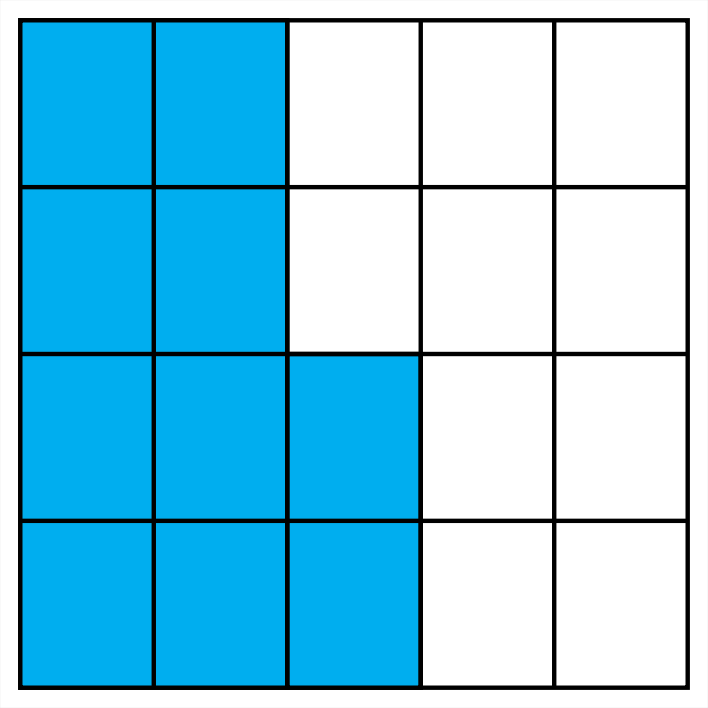
\includegraphics[width=45px]{../images/imagen_frac01.png} \fillin[\fbox{$\dfrac{10}{20}$}][0in] \\[1em]
				\part 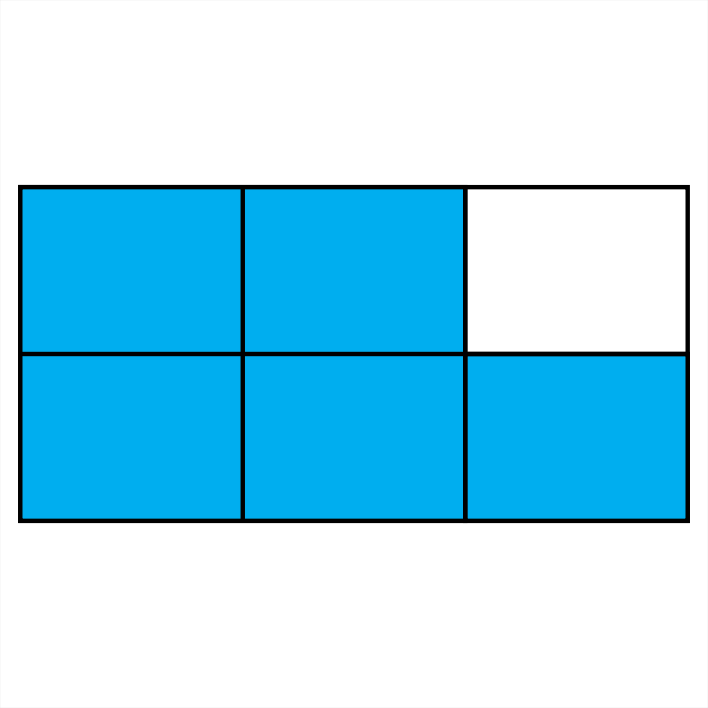
\includegraphics[width=45px]{../images/imagen_frac02.png} \fillin[\fbox{$\dfrac{5}{6}$}][0in] \\[1em]
				\part 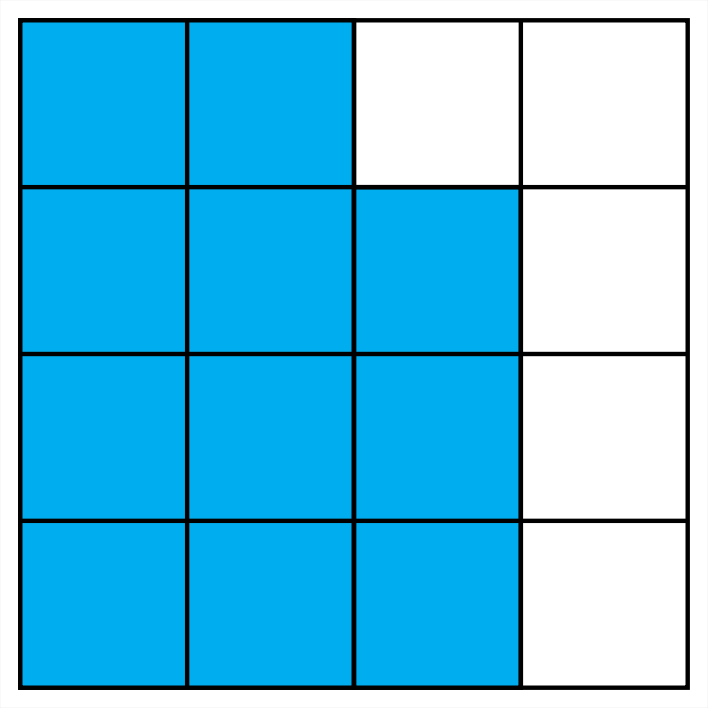
\includegraphics[width=45px]{../images/imagen_frac03.png} \fillin[\fbox{$\dfrac{11}{16}$}][0in] \\[1em]
				\part 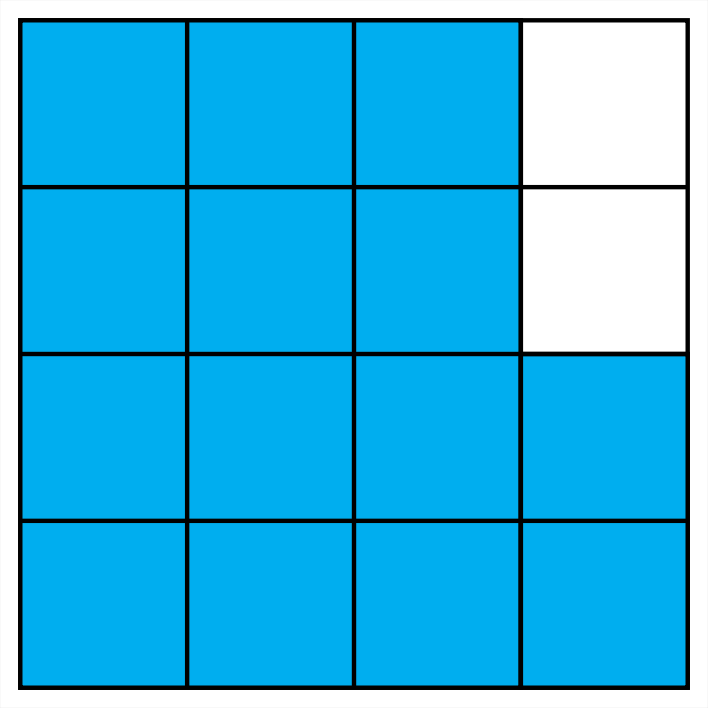
\includegraphics[width=45px]{../images/imagen_frac04.png} \fillin[\fbox{$\dfrac{14}{16}$}][0in] \\[1em]
				\part 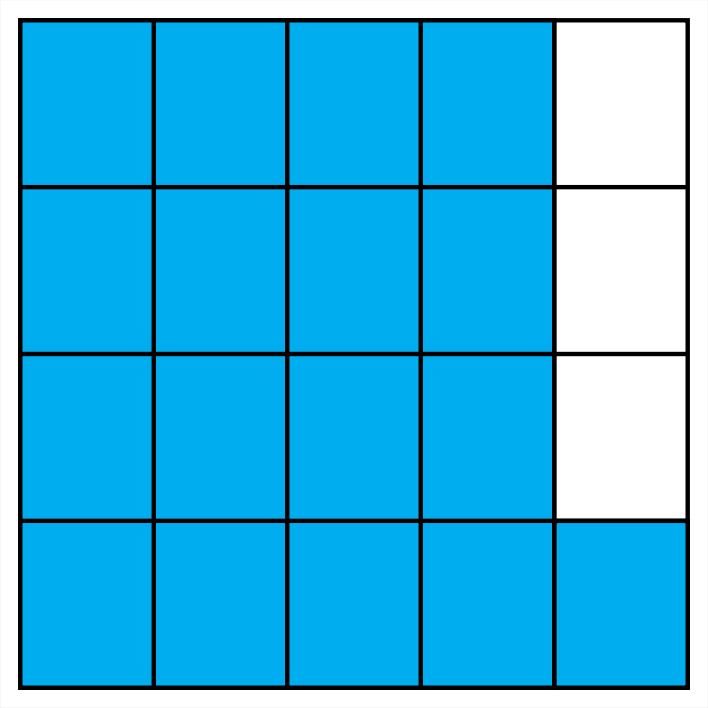
\includegraphics[width=45px]{../images/imagen_frac05.png} \fillin[\fbox{$\dfrac{17}{20}$}][0in] \\[1em]
				\part 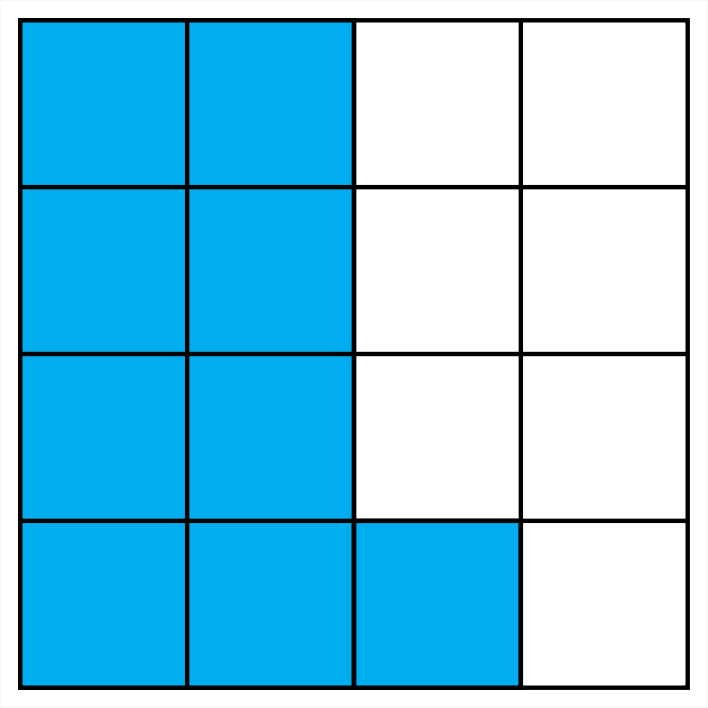
\includegraphics[width=45px]{../images/imagen_frac06.png} \fillin[\fbox{$\dfrac{9}{16}$}][0in] \\[1em]
				\part 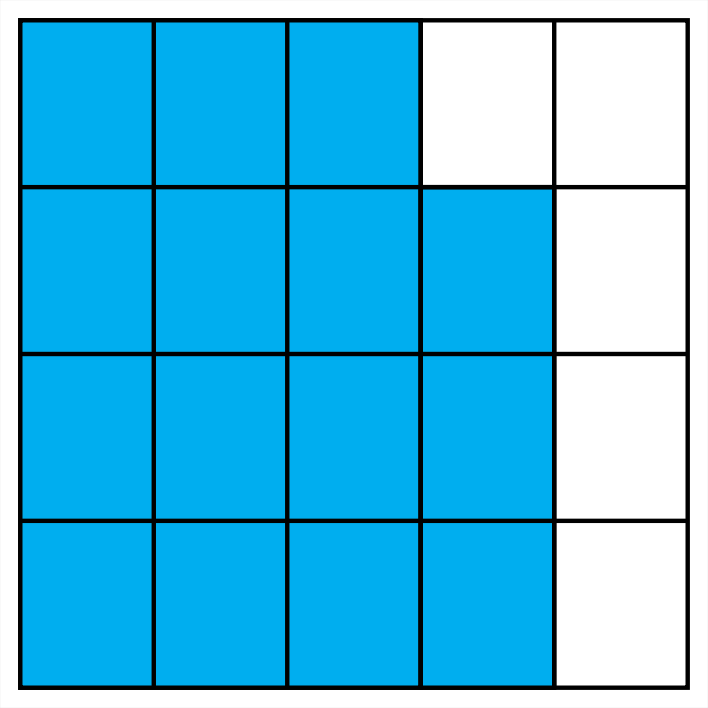
\includegraphics[width=45px]{../images/imagen_frac07.png} \fillin[\fbox{$\dfrac{15}{20}$}][0in] \\[1em]
				\part 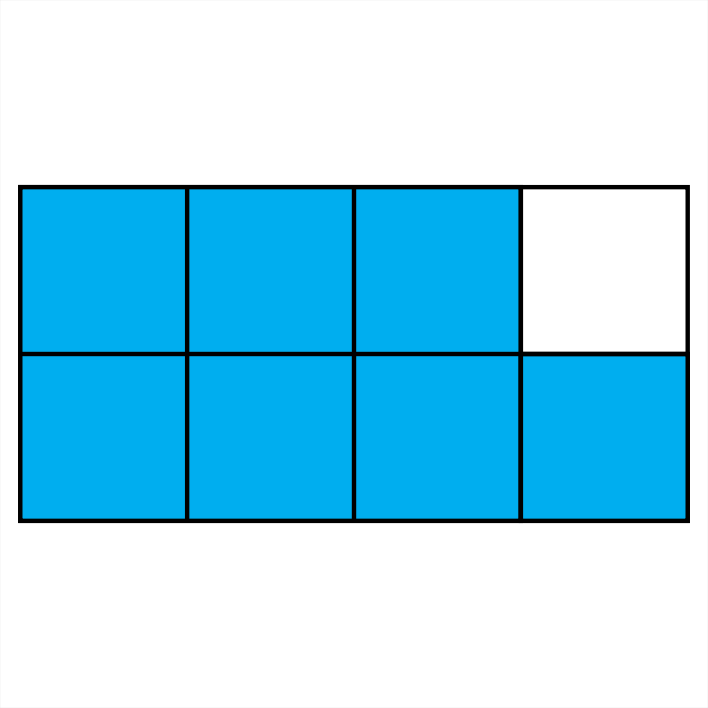
\includegraphics[width=45px]{../images/imagen_frac08.png} \fillin[\fbox{$\dfrac{7}{8}$}][0in] \\[1em]
				\part 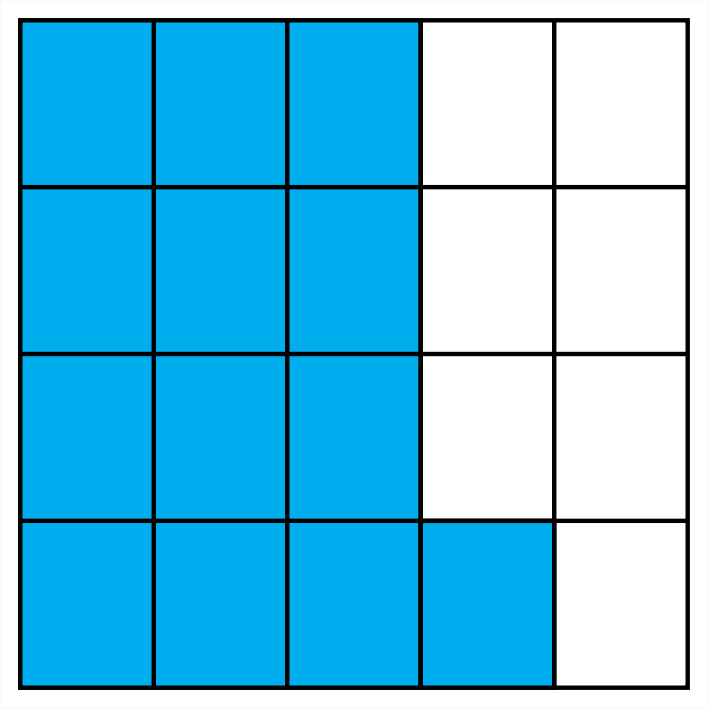
\includegraphics[width=45px]{../images/imagen_frac09.png} \fillin[\fbox{$\dfrac{13}{20}$}][0in] \\[1em]
				\part 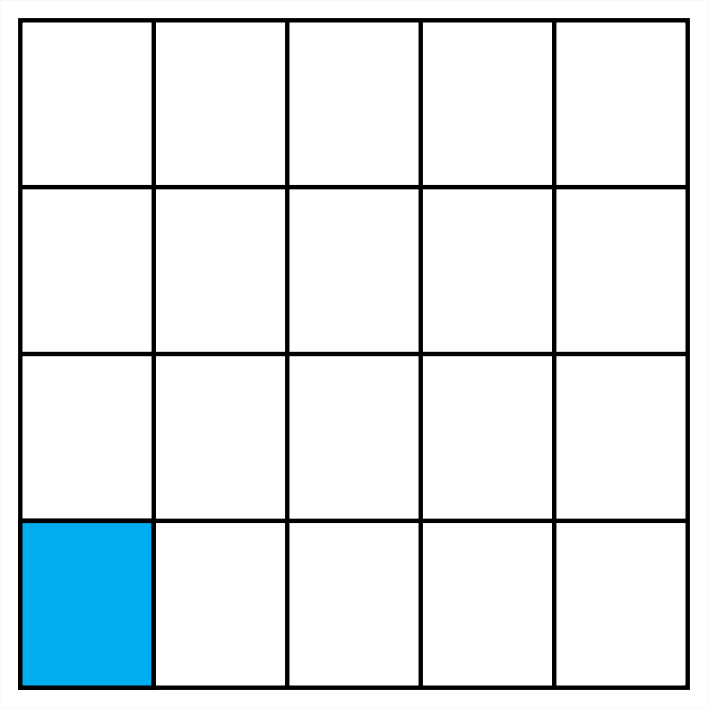
\includegraphics[width=45px]{../images/imagen_frac11.png} \fillin[\fbox{$\dfrac{1}{20}$}][0in] \\[1em]
			\end{parts}
		\end{multicols}
	}


	% \subsection*{\ifprintanswers{Nombre de fracciones                       }\else{}\fi}

	\questionboxed[2]{Escribe la fracción que corresponda en cada inciso:

		\begin{parts}
			\part ¿Cómo se escribe numéricamente la fracción \textbf{ocho quintos}?    \fillin[$\dfrac{8}{5}$][0in]  \\
			\part ¿Cómo se escribe numéricamente la fracción \textbf{seis onceavos}?   \fillin[$\dfrac{6}{11}$][0in] \\
			\part ¿Cómo se escribe numéricamente la fracción \textbf{dos séptimos}?    \fillin[$\dfrac{2}{7}$][0in]  \\
			\part ¿Cómo se escribe numéricamente la fracción \textbf{once medios}?     \fillin[$\dfrac{11}{2}$][0in] \\
			\part ¿Cómo se escribe numéricamente la fracción \textbf{diez décimos}?    \fillin[$\dfrac{10}{10}$][0in]\\
		\end{parts}
	}

	% \subsection*{\ifprintanswers{Conversión de fracciones mixtas a impropias}\else{}\fi}
	\questionboxed[4]{Convierte la siguientes fracciones mixtas a impropias:

		\begin{multicols}{3}
			\begin{parts}\large
				\part $4\dfrac{2}{3}= $ \fillin[$\dfrac{14}{3}$][0in]
				\part $2\dfrac{3}{10}= $ \fillin[$\dfrac{23}{10}$][0in]
				\part $5\dfrac{1}{5}= $ \fillin[$\dfrac{26}{5}$][0in]
			\end{parts}
		\end{multicols}
	}


	% \subsection*{\ifprintanswers{Conversión de fracciones impropias a mixtas}\else{}\fi}

	\questionboxed[4]{Convierte la siguientes fracciones impropias a mixtas:

		\begin{multicols}{3}
			\begin{parts}\large
				\part $\dfrac{13}{3}= $ \fillin[$4\dfrac{1}{3}$][0in]
				\part $\dfrac{63}{10}= $ \fillin[$6\dfrac{3}{10}$][0in]
				\part $\dfrac{51}{5}= $ \fillin[$10\dfrac{1}{5}$][0in]
			\end{parts}
		\end{multicols}
	}

	% \section*{\ifprintanswers{Operaciones con fracciones                 }\else{}\fi}
	% \subsection*{\ifprintanswers{Suma de fracciones                         }\else{}\fi}
	% \subsection*{\ifprintanswers{Resta de fracciones                        }\else{}\fi}
	% \subsection*{\ifprintanswers{Multiplicación de fracciones               }\else{}\fi}
	% \subsection*{\ifprintanswers{División de fracciones                     }\else{}\fi}
	% \subsection*{\ifprintanswers{Operaciones de fracciones mixtas           }\else{}\fi}

	\questionboxed[15]{Realiza las siguientes operaciones.

		\begin{multicols}{2}
			\begin{parts}\large
				\part $\dfrac{3}{10}+\dfrac{4}{5}=$ \fillin[$\dfrac{11}{10} = 1\dfrac{1}{10}$][0in] \\[0.75em]
				\part $\dfrac{3}{4}-\dfrac{2}{5}=$ \fillin[$\dfrac{7}{20}$][0in] \\[0.75em]
				\part $\dfrac{2}{3}-\dfrac{2}{5}=$ \fillin[$\dfrac{4}{15}$][0in] \\[0.75em]
				\part $\dfrac{3}{8}+\dfrac{7}{10}=$ \fillin[$\dfrac{43}{40} = 1\dfrac{3}{40}$][0in] \\[0.75em]
				\part $\dfrac{3}{5}\times\dfrac{2}{3}=$ \fillin[$\dfrac{6}{15}$][0in]   \\[0.75em]
				\part $\dfrac{7}{8}\times\dfrac{3}{4}=$ \fillin[$\dfrac{21}{32}$][0in] \\[0.75em]
				\part $\dfrac{3}{5} \divisionsymbol\dfrac{2}{3}=$ \fillin[$\dfrac{9}{10}$][0in] \\[0.75em]
				\part $\dfrac{7}{8} \divisionsymbol\dfrac{3}{4}=$ \fillin[$\dfrac{28}{24}$][0in]	\\[0.75em]
			\end{parts}
		\end{multicols}
	}

	% \section*{\ifprintanswers{Figuras geométricas                        }\else{}\fi}
	% \subsection*{\ifprintanswers{Nombre de figuras                          }\else{}\fi}
	% \subsection*{\ifprintanswers{Elementos de figuras                       }\else{}\fi}

	\questionboxed[2]{Escribe sobre la línea el nombre que recibe cada figura geométrica de acuerdo con su número de lados:

		\begin{multicols}{3}
			\begin{parts}
				\part 
\includegraphics[width=75px]{../images/pentagono_azul.png}  \fillin[pentágono][0.75in]
				\part 
\includegraphics[width=75px]{../images/nonagono_azul.png}   \fillin[nonágono][0.75in]
				\part 
\includegraphics[width=75px]{../images/decagono_azul.png}   \fillin[decágono][0.75in]
				\part 
\includegraphics[width=75px]{../images/hexagono_azul.png}   \fillin[hexágono][0.75in]
				\part 
\includegraphics[width=75px]{../images/rectangulo_azul.png} \fillin[rectángulo][0.75in]
				\part 
\includegraphics[width=75px]{../images/cuadrado_azul.png}   \fillin[cuadrado][0.75in]
			\end{parts}
		\end{multicols}
	}


	% \subsection*{\ifprintanswers{Perímetros 1                               }\else{}\fi}
	% \subsection*{\ifprintanswers{Perímetros 2                               }\else{}\fi}

	\questionboxed[4]{Contesta las preguntas sobre perímetros de figuras geométricas

		\begin{multicols}{2}
			\begin{parts}\large
				% \part ¿Cuál es el perímetro de un rectángulo cuya base mide 15 y su altura mide 6?

				% \begin{solutionbox}{1cm}
				% 	\[P=15+6+15+6=\color{red}42\]
				% \end{solutionbox}

				\part ¿Cuál es el perímetro de un rectángulo cuya base mide 38 y su altura mide 19?

				\begin{solutionbox}{1cm}
					\[P=38+19+38+19=\color{red}114\]
				\end{solutionbox}

				\part ¿Cuál es el perímetro de un cuadrado que sus lados miden 5?

				\begin{solutionbox}{1cm}
					\[P=5+5+5+5=\color{red}20\]
				\end{solutionbox}

				\part ¿Cuál es el perímetro de un pentágono que sus lados miden 18?

				\begin{solutionbox}{1cm}
					\[P=18 \times 5=\color{red}90\]
				\end{solutionbox}

				% \part ¿Cuál es el perímetro de un octágono que sus lados miden 15?

				% \begin{solutionbox}{1cm}
				% 	\[P=15 \times 8=\color{red}120\]
				% \end{solutionbox}

				\part ¿Cuál es el perímetro de un rombo que sus lados miden 16?

				\begin{solutionbox}{1cm}
					\[P=16 \times 4=\color{red}64\]
				\end{solutionbox}

			\end{parts}
		\end{multicols}
	}

	% \subsection*{\ifprintanswers{Área de figuras                            }\else{}\fi}

	\questionboxed[4]{Contesta las preguntas sobre áreas de figuras geométricas

		\begin{multicols}{2}
			\begin{parts}\large
				\part ¿Cuál es el área de un triángulo cuya base mide 18 y su altura mide 11?

				\begin{solutionbox}{1.5cm}
					\[P=\dfrac{18 \times 11}{2}=\color{red}99\]
				\end{solutionbox}

				\part ¿Cuál es el área de un cuadrado que sus lados miden 29?

				\begin{solutionbox}{1.5cm}
					\[P=29 \times 29=\color{red}841\]
				\end{solutionbox}
			\end{parts}
		\end{multicols}
	}
	% \section*{\ifprintanswers{Sistema de unidades                        }\else{}\fi}
	% \subsection*{\ifprintanswers{Reloj                                      }\else{}\fi}
	% \subsection*{\ifprintanswers{Multiplicaciones por múltiplos de 10       }\else{}\fi}

	\questionboxed[3]{Realiza las siguientes operaciones:

		\begin{multicols}{3}
			\begin{parts}\large
				\part $ 55 \times 10000=$   \fillin[550000][0.5in]
				\part $ 135 \times 100=$   \fillin[13500][0.5in]
				\part $ 369 \times 10000=$   \fillin[3690000][0.5in]
				\part $ 88 \times 10=$   \fillin[880][0.5in]
				\part $ 1215 \times 100=$   \fillin[121500][0.5in]
				\part $ 300 \times 10000=$   \fillin[3000000][0.5in]
				\part $ 224 \times 1000=$   \fillin[224000][0.5in]
				\part $ 13 \times 1000=$   \fillin[13000][0.5in]
				\part $ 134 \times 100000=$   \fillin[13400000][0.5in]
				\part $ 188 \times 10=$   \fillin[1880][0.5in]
				\part $ 401 \times 1000=$   \fillin[401000][0.5in]
				\part $ 42 \times 10=$   \fillin[420][0.5in]
				\part $ 92 \times 1000=$   \fillin[92000][0.5in]
				\part $ 1050 \times 1000=$   \fillin[1050000][0.5in]
				\part $ 19 \times 100=$   \fillin[1900][0.5in]
			\end{parts}
		\end{multicols}
	}



	% \subsection*{\ifprintanswers{Unidades de tiempo                         }\else{}\fi}
	% \subsection*{\ifprintanswers{Unidades de longitud                       }\else{}\fi}

	\questionboxed[3]{Realiza las siguientes conversiones de unidades de longitud:

		\begin{multicols}{2}
			\begin{parts}
				\part De 157 kilómetros a hectómetros. \hfill \fillin[1570][0.6in] hm \\
				\part De 25 centímetros a milímetros.  \hfill \fillin[250][0.6in] mm \\
				\part De 27 kilómetros a decámetros.   \hfill \fillin[2700][0.6in] Dm \\
				\part De 17 kilómetros a hectómetros.  \hfill \fillin[170][0.6in] hm \\
				\part De 69 kilómetros a centímetros.  \hfill \fillin[6900000][0.6in] cm \\
				\part De 59 decímetros a centímetros.  \hfill \fillin[590][0.6in] cm \\
				\part De 26 metros a decímetros.       \hfill \fillin[260][0.6in] dm \\
				\part De 4 kilómetros a milímetros.    \hfill \fillin[4000000][0.6in] mm \\
				\part De 135 kilómetros a decámetros.  \hfill \fillin[13500][0.6in] Dm \\
				\part De 112 kilómetros a hectómetros. \hfill \fillin[1120][0.6in] hm \\
			\end{parts}
		\end{multicols}
	}


	% \subsection*{\ifprintanswers{Unidades de masa 	                          }\else{}\fi}
	\questionboxed[3]{Realiza las siguientes conversiones de unidades de longitud:

		\begin{multicols}{2}
			\begin{parts}\large
				\part De 205 gramos a decigramos    \hfill \fillin[2050][0.5in] dg \\
				\part De 25 kilogramos a gramos     \hfill \fillin[25000][0.5in] g \\
				\part De 58 kilogramos a gramos     \hfill \fillin[58000][0.5in] g \\
				\part De 45 decagramos a gramos     \hfill \fillin[450][0.5in] g \\
				\part De 134 gramos a decigramos    \hfill \fillin[1340][0.5in] dg \\
				\part De 282 gramos a miligramos    \hfill \fillin[282000][0.5in] mg \\
				\part De 117 decagramos a gramos    \hfill \fillin[1170][0.5in] g \\
				\part De 17 decigramos a miligramos \hfill \fillin[1700][0.5in] mg \\
				\part De 115 gramos a centigramos   \hfill \fillin[11500][0.5in] cg \\
				\part De 62 gramos a miligramos     \hfill \fillin[62000][0.5in] mg \\
			\end{parts}
		\end{multicols}
	}

\end{questions}
\end{document}